\section{Pulse Width Modulation (PWM)}\label{afs:PWM}
På den diskrete version er CHARGE og DISCHARGE MOSFET'erne er altid tændte, såfremt en fejlsituation ikke er tilstede. For at detektere en fejlsituation skal en reference sættes, således at den maksimale op- og afladestrøm er veldefineret. PWM bliver ikke brugt i den integrerede version. \\

Referencen for den maksimale afladestrøm sættes ved hjælp af et PWM signal på $R4$ i schematic. Et PWM signal er nødvendig for systemets modularitet, da dennes værdi i softwaren kan ændres, hvorimod en reference opnået gennem for eksempel en spændingsdeler er fastlagt. Referencen for afladestrømmen udregnes i afsnit \ref{sec:overcurrent_dsg} til $1.7\volt$. Ligeledes bliver opladestrømmens reference udregnet i \ref{sec:overcurrent_chg} til at være $300\milli\volt$. PWM signalerne til referencerne genereres på følgende måde. \\

Der tages udgangspunkt i PWM signalet til kontrol af afladefetten, dvs. 1,7V. Duty cyclen udregnes: 

\begin {equation}
D = \frac{1.7\volt}{3.3\volt} = 0.515
\label{eq:duty}
\end {equation}

Da CTIMER'eren bruges til generering af PWM er opsætningen i grove træk det samme som beskrevet i afsnit \ref{afs:CTIMER}, dog med enkelte undtagelser. 

\begin{figure}[h]
	\centering
	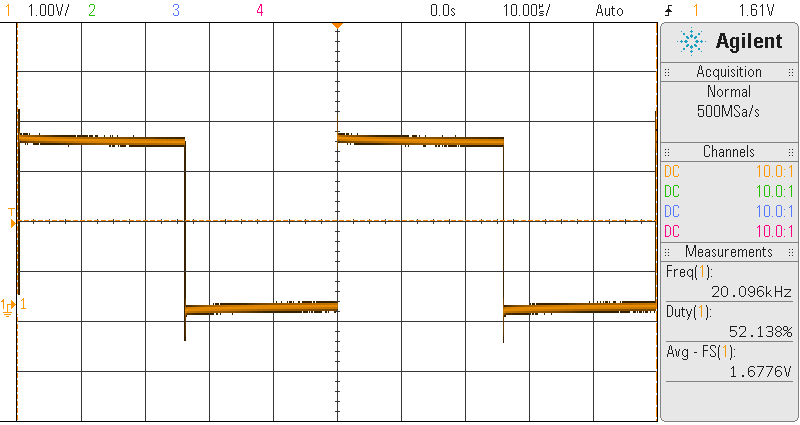
\includegraphics[width=15cm]{billeder/pwm_scope.png}
	\caption{Screenshot fra oscilloskop af PWM signalet}
	\label{fig:pwm_scope}
\end{figure}

%\verb|MIN_PACK_VOLTAGE|

\sbf{formel og kode}



Da sikkerheden ved overstrøm har en hysterese, skal en reset mulighed realiseres. Dette gøres ved at sætte dutycyklen til 100\percent\space og derved sætte en puls på $3.3\volt$ ind på reference benet. I tilfælde af for høj eller for lav temperatur sættes dutycyklen til 0\percent, for at slukke for MOSFET'erne.

